
\documentclass[sigconf]{acmart}

\usepackage{todonotes}
\usepackage{hyperref}

\usepackage{endfloat}
\renewcommand{\efloatseparator}{\mbox{}} % no new page between figures

\usepackage{booktabs} % For formal tables

\settopmatter{printacmref=false} % Removes citation information below abstract
\renewcommand\footnotetextcopyrightpermission[1]{} % removes footnote with conference information in first column
\pagestyle{plain} % removes running headers

\begin{document}
\title{Mapping Police Killing of Citizens in the United States}

\author{Jeramy Townsley}
\orcid{1234-5678-9012}
\affiliation{%
  \institution{IUPUI}
  \streetaddress{425 University Ave}
  \city{Indianapolis} 
  \state{Indiana} 
  \postcode{46202}
}
\email{jtownsle@indiana.edu}


\begin{abstract}
With the rise of camera phones that allows citizens to videotape law enforcement brutality against citizens, and the ability to immediately make those videos public through social media, there has been an increased awareness of police killings of citizens.  With this new data there have been a number of systematic attempts to document these events, from journalists, to academics, to activists, since there is no credible government database documenting this problem. These events can be mapped at the county level with the open source software QGIS.  Further, demographic and economic data gathered by the Census at the county level can be collected and tested against the police-killings to determine if a regression model can be used to describe a pattern among these variables. 
\end{abstract}

\keywords{i523, hid347, police violence, negative binomial regression, gis mapping, American Community Survey}

\maketitle

\section{Introduction}

In an era of seemingly ubiquitous tracking of human behavior by  overlapping layers of government, one would presume there would be reliable data on one of the worst possible crimes--homicide. Further, one would presume, that in a democratic society, where government transparency and the fundamental importance of civil liberties dictates limits on the state's ability to take the lives of its citizens, that record-keeping of state-inflicted deaths would be meticulously collected and curated. \cite{brucato15} However, in both cases, the data that is publicly available through government databases is significantly incomplete.  \cite{currie16, pridemore05,dalton17,nix17} For example, the {\em Washington Post's} project to collect data on police killings for 2016 claims to have more than twice the number of such deaths than are recorded in FBI statistics. \cite{fatalforce}  Other projects with the same goal have found similar results. \cite{policeviolence,counted} 

Journalists have taken the lead in finding ways to collect national databases of police-inflicted deaths and to create easy ways for the public to access those resources. \cite{currie16,nix17,counted,fatalforce} They are doing so using some of the tools of big data, such as combing the internet for daily references to such events, then plugging that data into ongoing projects.  Last year alone there were over 1,000 killings of U.S. citizens by police. \cite{counted}  With that data, other types of analysis can be done, such as mapping, and statistical models that relate predictor variables to differing rates of law-enforcement fatal violence.  Since journalist efforts have produced, in most cases, the exact address where each killing has occurred, the possibility of geocoding each event for advanced geospatial analysis is possible. \cite{dalton17}  Similarly, since the geographic locations are known, other types of data, such as demographic, economic and political data can be used as potential predictor variables. \cite{smith04,legewie15}

While it is not known whether there has been an increase in citizen deaths caused by police in the last few  years, because of the unreliability of data about these incidents, there has been an increased awareness in the general population of the extent of these killings, arguably brought to the public's attention by the availability of social media, and easy access to filming and photographing equipment through the cameras on smart-phones, carried by a significant percent of the public. \cite{bonilla15,brucato15,nix17}  Regardless, the issue of police brutality and particularly police killings has inspired movements such as Black Lives Matter to specifically highlight these issues, not only for people of color, but for all citizens.  While these efforts largely became national movements after the killing of Michael Brown by police officer Darren Wilson, in Ferguson, MO, in 2014, scholars had already been looking into how to understand the extent of these killings, along with other types of police use of excessive force against citizens. \cite{smith04,smith14,meeks06,schneider14,chaney13,holmes00}  

The success of these movements in facilitating national dialogues about these issues, and available research on police brutality, create a foundation on which public police may be constructed to minimize these outcomes, which are unique to the United States. Among all high-income countries, the US alone has rates of citizen deaths due to law enforcement above 0.5 people killed by police gunfire per million residents.  While U.S. police shot to death 3.1 people per million, police in the next highest industrialized country, Australia, shot only 0.21 people per million, and Denmark was next, at 0.18 people per million.  \cite{ser16}  According to reporting on this issue in {\em The Guardian}, police in England and Wales have shot to death 55 residents in the last 24 years, while in the United States, police have shot to death 59 residents in the first 24 days of 2015. \cite{lartey15} 

\section{Police Use of Excessive Force, and Deaths Caused by Law Enforcement}
The National Violent Death Reporting System, created by the Centers for Disease Control, and  in a sample of seventeen participating states, tracks all reported violent deaths in those locations.  In 2013 they report that about 1.2\% of all violent deaths were caused by law enforcement, and non-Hispanic Black men were four times as likely as White men to be victims of law enforcement-caused deaths (as a percent of the population). \cite{cdc13}  From multiple years of CDC data, this seems to be relatively consistent over the time of study.  

Scholars, journalists and activists have noted both the rates of U.S. law-enforcement deaths compared to other industrialized countries, and the lack of reliable government data on the national number of such killings. \cite{currie16,pridemore05,dalton17,lartey15,ser16}  While journalists, the FBI, and the CDC have been documenting basic counts and demographics of residents killed by police, scholars have tended to explore various theoretical frameworks that can make sense of these patterns.  Most of these fall into a few categories: race-specific, individualistic, situational, organizational, and ecological. \cite{nix17,provine11,smith14,chaney13}

\subsection{Theories of Police Violence}
Race-specific theories build on a long history of critical race studies documenting racial inequality in the United States, from slavery until today. \cite{provine11,chaney13,meeks06,crichlow14,payne17}  These approaches explore concepts like structural racism, implicit bias, discrimination, segregation, the prison-industrial complex, and economic disenfranchisement.  In terms of interactions with the legal system, critical race theory argues that race minorities are often targeted specifically because of race, tracing back to the slave-era days, to the era of lynchings, and to today where data indicates higher rates of conviction and imprisonment for race minorities, and higher rates of the use of excessive force by police against race minorities.  \cite{payne17,provine11,meeks06,chaney13,crichlow14,petro03}  

A specific variant of this approach explores the social psychological effect of inter-group threat perceptions.  The minority threat hypothesis proposes that very small groups of race minorities pose little economic or political threat to the majority.  However, once a critical threshold is reached, the majority perceives significant threat from the minority group, and deploys various tactics to try to neutralize that threat, such as discriminatory housing policy, increased used of police as a tool for economic extraction and political violence, education discrimination, and employment discrimination. \cite{luders10} Conversely, a parabolic curve is predicted, such that once the minority population grows above 50\%, they have sufficient political power over time to counter these patterns. While some early research found only mixed evidence to support the minority threat hypothesis, the majority since have shown significant support. \cite{legewie15,smith04,smith14,holmes00,stults07,jacobs02,kent05,petro03}  Further, from subsequent reanalysis of studies that did not show robust minority threat effects, it is argued that the earlier efforts examined raw population numbers, but once proportionate shares of the population were used instead, significant effects were found. \cite{legewie15}

Other theoretical approaches do not focus on issues of race, as such.  For example, the individual approach argues there are specific characteristics of police that lead some to be more likely to kill citizens.  Various characteristics have been studies, such as level of education, implicit bias (related to a race-approach, but on an individual level), professionalism, and personality traits.  \cite{nix17,smith04}  There is mixed to low support for any individual characteristic.  Similarly, the organizational approach has mixed to low support.  Organizational characteristics proposed to be related to police use of excessive or deadly force are an increased bureaucracy, more stringent entrance requirements, higher levels of training, and greater levels of community accountability. \cite{nix17,smith04,smith14} A counter-intuitive finding that seems to be consistent, is that higher levels of training can actually lead to higher levels of police violence, although there was little evidence to support a specific cause.

Situational theories propose that there is something specific in the interactions between police and those they kill that led to the deadly force.  Some evidence supports the conclusion that hostile, armed, or impaired suspects are more likely to be victims of police violence or be killed by police.  \cite{nix17}  However, evidence also suggests that a history of police brutality against people of color, as well as over-policing specific to communities of color, significantly increases the likelihood that race minorities will be more suspicious of law enforcement, and thus less willing to cooperate. \cite{payne17,kent05} Finally, ecological theories argue that levels of community violence, spatial organization, and community inequality are related to police violence.  For example, evidence shows that in communities with higher crime rates, especially higher rates of homicide, police are more likely to use excessive force, and suspects are more likely to be killed by police. \cite{nix17,smith04,smith14}  Similarly, communities experiencing economic deprivation and inequality have been found to experience higher rates of police violence and police killings. \cite{jacobs02,meeks06,stults07,legewie15,payne17}

\section{Tracking Deaths Caused by Law Enforcement}
There is no central database in the United States for any killings, whether caused by citizens or law enforcement.  The best publicly available government resource is the FBI database on homicides from the Uniform Crime Report (UCR).  However, as numerous sources have documented, this database is unreliable because participation by local and state law enforcement agencies is voluntary. \cite{currie16,pridemore05,dalton17} There have been several attempts by researchers and law enforcement to get a better picture of homicide rates.  For example, the FBI's Supplementary Homicide Report, and National Vital Statistics Systems are two federal-level attempts to collect more detailed statistics, but those efforts are not presumed to represent the entire population of homicides. \cite{pridemore05}  Similarly, the Centers for Disease Control collected a sample database, originally of just seventeen participating states in 2013, the National Violent Death Reporting System, cataloguing various aspects of all reported violent deaths, including whether law enforcement was involved. \cite{cdc13}  Each of these is not a full-scale national survey, but small samples.  However, what they all show is the failure of the UCR to capture even a majority of law enforcement-caused deaths.

Similarly, data on homicides specifically reported to have been committed by law enforcement face similar deficits.  \cite{currie16,pridemore05,nix17}  To overcome this problem, journalists, academics, and activist organizations have used publicly available sources to find instances of law enforcement-caused deaths.  For example, the British news agency, {\em The Guardian}, created a two-year project, The Counted, where they manually searched news reports for cases of deaths caused by law enforcement.  \cite{counted}  Additionally, they posted contact information for the public to send them tips about cases not already in their database.  While The Guardian database for 2015-2016 remains available to the public, they discontinued the project, so no 2017 data is available.  It has some interactive features, where the user can filter the data by state where the killing occurred, how the death occurred, whether the victim was alleged to have been armed, victim's gender, race, and age.  Where possible, a picture of the victim and a brief biography is available.  They report that 1,093 people were killed by law enforcement in 2016 alone.

Another new agency that relies on a similar process to capture data about deaths caused by police, is the {\em Washington Post}.  They host an ongoing project that lists only people shot to death by police, Fatal Force, and contains links to the original news stories where the deaths were reported. \cite{fatalforce}  Its numbers are lower than The Counted, which includes any deaths caused by law enforcement, not just shootings.  However, it also notes that its database has more than twice the number of shootings by law enforcement per year than the FBI database.  Like {\em The Guardian}, it has contact information to send new information about killings, as well as photos or videos about the victims.  Their list of victims starts from January 1, 2015.  They report that 963 people were shot to death by law enforcement in 2016.

Mapping Police Violence (MPV) was created by three community activists and organizers.  Their reported methodology is to have used three online databases, and to have compiled those lists into MPV.  Neither {\em The Guardian} or the {\em Washington Post} are reported as a source for MPV for the two years of data available from those agencies. They operationalize police killings as, ` case where a person dies as a result of being chased, beaten, arrested, restrained, shot, pepper sprayed, tasered, or otherwise harmed by police officers, whether on-duty or off-duty, intentional or accidental.' \cite{policeviolence} Their list of victims begins from January 1, 2013.  They report that 1155 people were killed by law enforcement in 2016.  This is the database used for this project to identify the counties where people were killed by law enforcement.

\section{Critical Studies, Counter-Mapping, and Counter-Data}
In addition to efforts at tracking law enforcement relate deaths, a broader movement has arisen in the era of big data, merging the scholarship and practice of critical studies with data science.  Specifically, some scholars and activists are discussing practices of counter-data, and counter-mapping, as an attempt to mitigate the state's use of big data and mapping to enlarge the carceral state. \cite{jefferson17,currie16,dalton17,ccc12}  This approach highlights how government and capitalism constructs a specific vision of the world that creates tight boundaries around civil liberties, rather than expanding civil liberties, which is arguably one of the original visions of a good society under liberalism

\subsection{Critical Studies, Foucault}
Critical studies began in the 1920s at the Institute for Social Research in Frankfurt, Germany, in response to the rise of fascism. \cite{ritzer18,seidman16}  Several key thinkers, such as Adorno, Horkheimer and Marcuse, tried to integrate neo-Marxism, Max Weber, and Freud, into a liberating sociology that rejected the growth of the oppressive state.  All of these early founders wrote and spoke vigorously against Hitler, and were eventually forced to flee Germany, transplanting critical studies to Columbia University. \cite{ritzer18}   Their outlook critiqued the current (at the time) emphasis in the social sciences of positivism, which seemed to strip the humanity out of social ideas, reducing people to the condition of biological robots.  Further, the growing efficiency and expansion of the state with the success of bureaucracy and the so-called `scientific management' of Frederick Taylor, society was increasingly treating people like the robots described by sociology and psychology.  Finally, the successful takeover by capitalism of all social processes, not only the economy, but a restructuring of how humans treated each other--as competitors, as sources of capital, and bodies to be exploited for labor--brought critical studies to critique the entire direction of society.  This approach contrasted with the Weberian approach that argued for neutral objectivity, not directly attempting to critique and change society. \cite{ritzer18,seidman16}

Subsequent to the original founders of critical studies, later thinkers built on these ideas.  Michel Foucault, a French scholar writing in the 1960s and 70s, produced a series of critiques of social structures, from an examination of the growth of prisons, to problematic psychiatric approaches at mental hospitals, to how cultural approaches to sexuality were often used as a specific form of social repression.  In contrast to the original critical theorists who built on Marx and Freud, Foucault rejected both of those approaches to understanding society.  Two of Foucault's methods he describes as archaeology of knowledge, and genealogy of power. \cite{ritzer18,seidman16}  Much as traditional archaeology is a process of digging into the past to see how an ancient society was built, Foucault's archaeology of knowledge was a process of digging into texts to discover how knowledge systems are built that then structures how a society operates and performs various discourses.  Similarly, much as a family genealogy traces back how individual people are related to each other, Foucault's genealogy traces back ideas to see how they are related to each other, and in doing so, describes ways to understand power in society, since knowledge in modern societies is a key to power.  

Foucault argues that if the leaders of a society can harness technologies to maximize their knowledge of members of that society (and they do), they can wield great power over those members.  For example, in {\em Discipline and Punish}, Foucault describes the concept of Panopticon, based on a prison design by Jeremy Bentham in 1791. Built in such a way so that the prisoners never knew when they were being watched by the guards, and they could easily be seen at all times, the idea was that they would eventually start to subjugate their own behaviors to the will of the prison guards, thus minimizing the efforts the prison had to take to control them--the prisoners disciplined themselves rather than having to be constantly disciplined and punished by the guards. \cite{foucault77}  Similarly, modern school rooms are typically structured such that the teacher stands at the front of the room, while student desks are in rows facing forward.  The teacher can easily visualize all students in one glance, and the students recognize they can be seen at any moment, and thus are more inclined to discipline their own behaviors.  Foucault argues that by simply creating a technology of ubiquitous observation, it radically reshapes citizen behaviors.  These issues became part of daily life under Stalin and Hitler, as hordes of citizens were conscripted into the government machinery as spies on their neighbors.  All aspects of citizens' daily lives were monitored, reported, documented, and if applicable, punished.

\subsection{Foucauldian Activists, Counter-Data}
Contemporary activists and scholars recognize the ways that Foucault's vision of a ubiquitous monitoring system can constrain human liberty.  Jefferson highlights this concern in a description of the Chicago Police Department's use of digital mapping for crime, CLEARmap, in a cleverly-titled article based on Foucault's essay, {\em Digitize and Punish}. \cite{jefferson17} Jefferson describes the fact that CLEARmap is not a neutral, objective mapping system, but is `provides ostensibly scientific ways of reading and policing negatively racialized fractions of surplus labor in ways that reproduces, and in some instances, extends the tentacles of carceral power.'  In doing so, Jefferson claims to be linking critical mapping (`critGIS'), and critical race/ethnic studies.  Because of how highly over-policed race-minority communities are, these are the regions most likely to have high concentrations of citizens pulled into the carceral state. \cite{gilbert15,brunson05,rios11,crichlow14,payne17,chaney13,schneider14} Thus, such mapping not only visualizes crime, but it also becomes a tool for racial subjugation, expanding police and state action in communities already over-policed.  Brayne explores the same concerns in a study of the Los Angeles Police Department. \cite{brayne17}

Currie, et al, summarize the field of counter-data, which incorporates critical studies with big data. \cite{currie16} Specifically, concerned about the lack of transparency of the various, overlapping layers of government as it relates to police brutality in communities, they argue that residents should use the tools available to them to construct their own data sets, thus creating leverage for greater government accountability.  This requires creating infrastructures for gathering, processing and distributing information to the public.  They note that government data on police brutality is widely recognized as flawed and grossly incomplete. \cite{currie16,patterson16,dalton17}  Noting that government data collection can be easily used to constrict citizen liberties, while at the same time, failing to protect citizens from the state, they point to counter-data as a process by which citizens collect their own data as a means of protection.  

Counter-mapping is an extension of counter-data, but applying the process of data-collection to how people think about the spatiality of the places around them.  Dalton and Stallman describe counter-mapping, which, `involves map-making practices by those outside of on the margins of large, powerful institutions such as corporations or governments. \cite{dalton17} The modern history of most maps and GIS is one of government programs, such as extending territory, military conflicts, property cadastres, or administering territories' (p. 3).  They point to activist mapping projects, such as Mapping Police Violence, as a way for citizens to map ways that the state imposes power unjustly, and package it into formats that are readily available to the public, thus empowering them as citizens by increasing their awareness of state practices. Similar citizen-activist mapping projects to oppose state imposition of power are described by the Maharawal, regarding gentrification in San Francisco, and the Counter Cartographies Collective, et al, describing counter-mapping as `militant research' that benefits the masses overtaken by an overreaching, exploitative state. \cite{maharawal17,ccc12}

\section{Data and Measures}
\subsection{Dependent Variable: Count of People Killed by Police}
The dependent variable is a count of the number of people killed in any given county in the United States from January 2013 to October 2017 and was downloaded from the web site, Mapping Police Violence (mappingpoliceviolence.org) on November 5, 2017.  Compared to the two news agencies that have been tracking deaths from law enforcement, their list of victims is more comprehensive for 2016 (1155 vs 963 and 1093), and it covers a longer time-frame, since the news agencies only have data since 2015.  The original downloadable xlsx (Excel) file contained 24 variables on the primary sheet, such as the victim's name, whether the victim was armed, a link to the original news story, whether there were reports of mental illness, the county, zip-code, state, specific address of the killing, victim's age, race, gender, date of the incident, and police department involved in the killing. At the time of download, the spreadsheet contained a total of 5,634 observations, that each represent a killing by law enforcement in the US in approximately the last five years.

This data contained errors that had to be manually corrected.  The errors were discovered when the "killed" variable, count of the number of people killed by law enforcement in any given county, was merged with the Census data that were the independent variables.  The Census data contains an official list of states and counties in those states. The MPV data listed counties that were not in the claimed states.  It was discovered that some were simply errors, some were city coded as county, and some were blank.  Sixty observations total were found to have errors.  Using the victim's name provided by MPV, they were searched using Google in November, 2017, to find an original news story reporting this killing.  Once the killing could be verified, similar investigation confirmed the county and state of the killing.  The corrected data was used for this analysis.  It is possible that other errors exist, since the only errors detected were those where there was no correct match with an actual Census-listed county and state.  There may be counties where a victim is claimed to have been killed, where the county and state exist, but misidentified.  The data has approximately the same number of observations as the two news agencies' data, strengthening its claims to validity.  Further, each of the 60 misspecified counties tracked back to an actual killing by law enforcement based on a search of the victim's name.

\subsection{Independent Variables: Census Data}
Summary statistics and definitions can be found in Table 1 for all of the variables used.  The independent variables were all obtained from the United States Census, which maintains a large, publicly-available database on their website. \cite{census}  All of the data used for this study are at the administrative unit of the county, and includes all of the 3142 United States counties listed by the Census.  All of the ten variables were downloaded (November, 2017) from the American Community Survey (ACS). The ACS is a subsidiary of the Census Bureau which administers an extensive survey of an annual sampling of the US population on various economic and demographic questions.  Each of the variables chosen for this project falls into one of five categories: population total, race, education, geography-type and economic.  The total population of each county is estimated by the ACS based on annual census data, and represents a single-year value.  The rest of the variables are estimated from aggregates of data collected from 2011-2015, a five-year estimate.  Multiple studies have shown that for homicide analysis, whether resident-on-resident killings, killings by police, or killings of police, demographic and economic variables tend to have strong predictive value. \cite{pridemore05,kaminski05,legewie15,patterson16,smith14}

\begin{table}
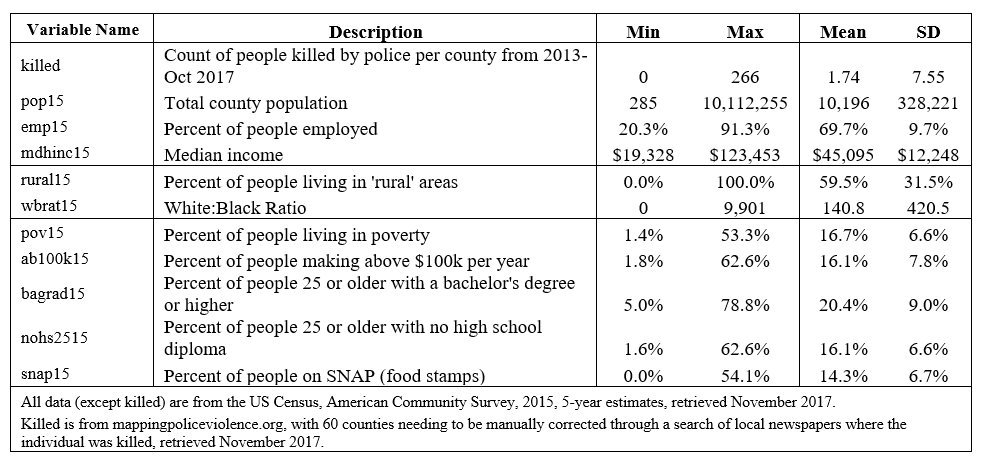
\includegraphics[width=1.0\textwidth]{images/table1.jpg}
\caption{All variables used in this study.}
\end{table}

The only race variable in this study is a ratio of White:Black population per county.  The Census uses self-identification of the individuals to label race.  Individuals can self-identify as multiple race and ethnic groups.  In this case, only those individuals listing a single race, White or Black, were counted, and a ratio was calculated.  The geography-type variable represents whether a person lives in a rural or urban area.  The census defines {\em urban} as any place with at least 2,500 people, and {\em rural} as everyplace else.  This variable is a percent of the county population who does not live in an urban area.  The two education variables only count those residents who are over 25 years of age, either who have a bachelor's degree or higher, or who do not have a high-school diploma.  

There are five economic-related variables.  The first, percent of people employed compared to the county population, is taken only from those 20-64 years old.  The second measures the median income per county.  Income can be measured in several different ways, and while mean is a common measure of central tendency, it is often skewed up by high incomes, since low incomes are limited to zero.  Because of this, median income is typically used.  Two variables measure income deficits--the percent of people who have qualified for SNAP (food stamps), and the percent of people living below poverty.  The latter relies on the definition of poverty provided by the Office of Management and Budget, which varies this designation based on size and composition of the family.  The fifth measure is the percent of the population living above \$100,000  per year. The Census lists the median U.S. income at almost \$60,000 per year, and provides the \$100k data as a measure of a high-income county.

\subsection{TIGER Shapefiles for Mapping}
In addition to demographic and economic data, the Census Bureau provides a significant amount of geospatial information.  Through their TIGER products (Topologically Integrated Geographic Encoding and Referencing), they provide a web site where the public can download shapefiles at many different levels that are published each year, and can be connected to the rest of their data. \cite{tiger} For this study, county-level data was used, since it was the smallest administrative unit for which all of the data was available.  While accurate state-level data was available, it did not seem fine-grained enough to provide a sufficient analysis.  Smaller administrative levels, like census-tract, and even block-level shapefiles are available, and there is annual census data that can be mapped onto those levels.  While some ACS variables are available at these small units, they typically only cover a random selection, and can have high error rates.  County-level data is the smallest administrative unit for which every county in the U.S. can be measured in the five-year estimates file.  The shapefile used for this study is the 2015 county-level data for the entire United States, and was downloaded from the Census TIGER site (November, 2017). \cite{tiger}  However, not all places available on the shapefile have data through the ACS.  For example, several of the smaller island territories are not included in the ACS survey, so those are excluded in the map, as well as the regression analysis.  While the latter includes Alaska and Hawaii, for ease of viewing the county-level data, those states are not included on the map (Figure 1).

\section{Methods}

There are multiple ways to attempt to understand police killings of citizens.  One way is by visualizing data of the events.  Another is by creating statistical models that relate the killings to predictor variables, such as in a regression equation.  Open source software is available for both of these approaches.

\subsection{Mapping, Quantum GIS}
Quantum GIS (QGIS) is open source software that facilitates the visualization of spatial information, and is useful for tasks such as mapping, and seeing how data are related in geographic ways. \cite{qgis} For this project, QGIS 2.18.8 was used to process the Census TIGER shapefile (shp) that contained all of the United States counties.  When downloading files from the TIGER site, several other files come with the shp file, one of which is a database file (dbf) that contains information about each place identified in the shapefile.  For example, land and water mass frequently come with the dbf, along with geocodes and names that identify specific locations. 

In this case, since it is a county-level datafile, the first entry in the dbf is Cuming County, Nebraska, with Nebraska geocoded as state \#31, and Cuming County geocoded as county \#039.  All 3142 counties in the dbf file have these coded identifiers that match spreadsheets of demographic and employment data that can be downloaded from the Census Bureau, such as the ACS data.  Since the geocodes are identical, this data and the shapefiles can be easily integrated.  Integrating other types of data, such as the police killings data from MPV, requires a different approach.  In this case, since MPV provided both the county and state names where the deaths occurred, merging these into one string, such as "CumingNE", and doing the same with the TIGER shapefile data, the two files can be joined.  For Figure 1, which shows the rates of killings by police at the county-level, a ratio was calculated in QGIS--the count of those killed in each county divided by the total population of that county.  With the creation of this new variable, it can be mapped in QGIS as a {\em graduated symbol} with a pre-specified color scheme. 

\begin{figure}
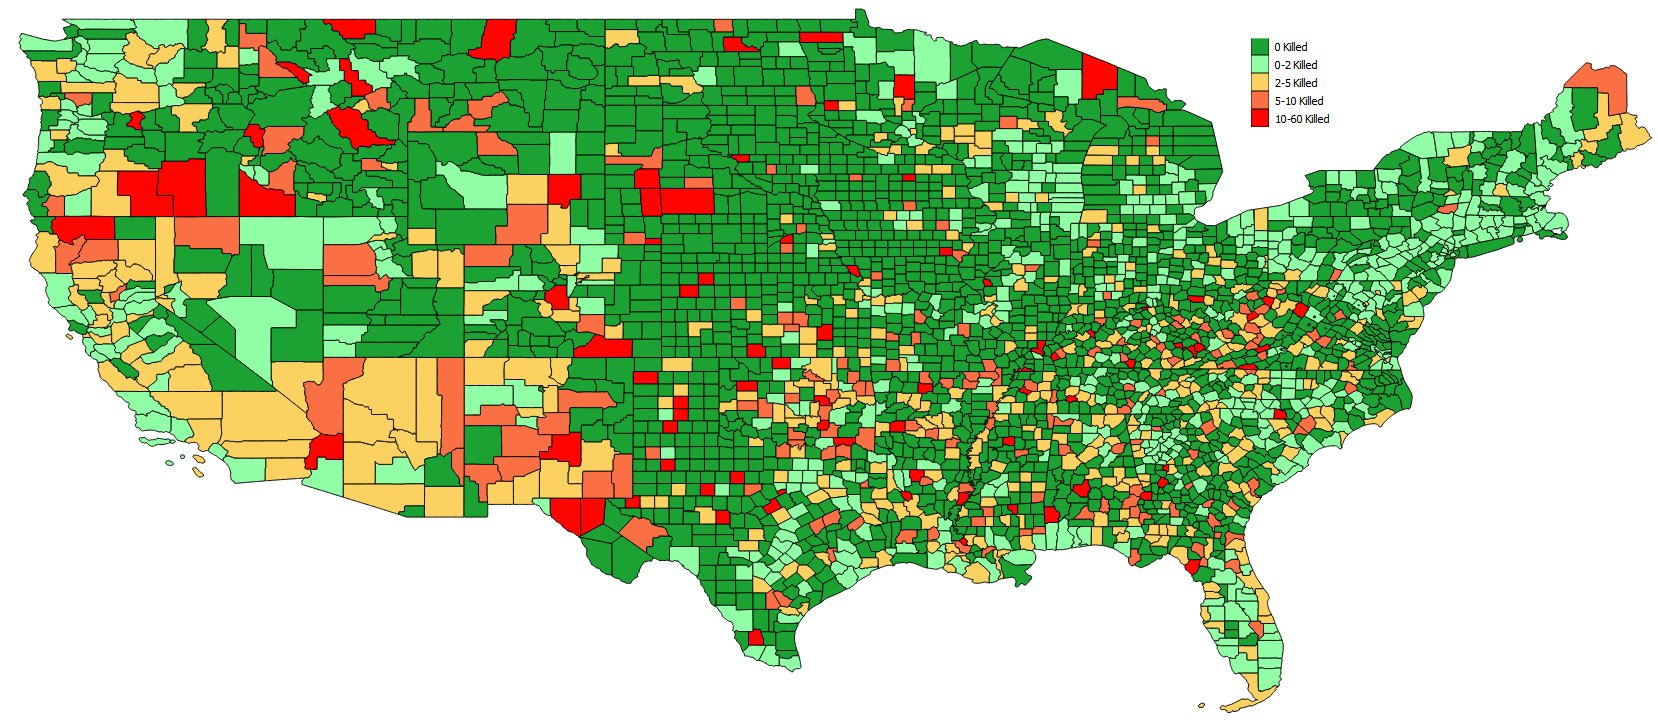
\includegraphics[width=1.0\textwidth]{images/figure1.jpg}
\caption{U.S. county-level map of residents killed by police, 2013-Oct 2017.  Data from Census and mappingpoliceviolence.org}
\end{figure}

This process can be automated with Python, a programming language useful for big data analysis. \cite{python}  QGIS has integrated Python into its software by including a Python Console for direct use, and an extensive instruction manual is available online through the QGIS web site. \cite{pyqgis}  For the map in Figure 1, a Python script was created that downloads a zipped file containing the TIGER shapefile for the US counties, and all of the census data that had previously been integrated into the dbf file. The script and data are available on the author's github course site. \cite{townsley} The zipped shapefile is available on the author's Indiana University Box account. \cite{townsley2} The Python program unzips the file, deletes all parts of the map except for the contiguous United States (all but 48 states), then applies a graduated color scheme to the killed/population ratio variable.

\subsection{Regression, Count Data and Data with a Mass at Zero}
Regression analysis and graphs can also be accomplished through open source software, R, an environment for statistical analysis and graphics. \cite{r}  In addition to the base R package, which is command line only, other packages are available as an overlay to incorporate GUI features, such as RStudio. \cite{rstudio}  This analysis was done with R 3.4.1, using RStudio 1.0.153.  Instead of Python, R has its own scripting language.  The R-script for the following procedures and data are available on the author's github course site. \cite{townsley}

Creating a statistical model is a way to understand how variables are related to each other.  Regression analysis is a common way to model such relationships.  While more typically used with a continuous dependent variable, regression can also be used to model count variables. \cite{kaminski05} In this case, the number of people killed by police is a count variable, and all of the predictor variables are continuous.  Modelling continuous dependent variables presumes a Gaussian distribution, but count variables often do not meet this assumption. \cite{fox15} While transforming a non-normal dependent variable is the typical procedure to get it into a state of normal distribution for analysis, using square root, reciprocal, log, or even a Box-Cox procedure, count variables can resist this process.  Poisson and negative binomial distributions are typically better suited for count data. \cite{martin17} These distributions can have an unusually large mass at zero, one of the prime reasons transformations fail. \cite{farewell17,beaujean16,gamlss,fox15,neelon16} 

Count data with a mass at zeros can be analyzed in a number of ways, depending on the theoretical reason for the zeros, each of which requires a different analytic approach.  One decision factor includes knowing whether there is one process generating all of your data, or whether there are two--one generating the count data (above zero) and some of the zero, and a second process generating {\em an excess} of zeros. \cite{neelon16,farewell17,min02,martin17}  In the latter case, these zeros would be more than would be predicted from the given distribution, and the are sometimes called {\em inaccessible} zeros.  Inaccessibility zeros are considered excessive, and a two-part, zero-inflated model might be a good option.  Zero-inflated Poisson, and zero-inflated negative binomial models are available in R, in packages such as {\emgamlss} and {\em pscl}. \cite{gamlss} The {\em killings by police per county} dependent variable is shown in a histogram, and as a plot against the county population, in Figure 2, both graphs being created in R using the standard {\em hist} and {\em plot} functions.  The large mass of zeros in the histogram might lead one to presume a zero-inflated model is most appropriate.

\begin{figure}
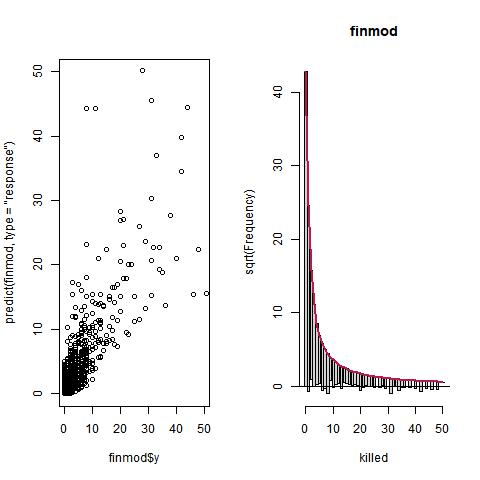
\includegraphics[width=1.0\textwidth]{images/figure2.jpg}
\caption{Left: Histogram of the number of county residents killed by police.  This histogram shows a maximum of eight per county killed by police, while the actual maximum is 266.  However, there are only 120 observations where this value is above 8.  This view gives a better depiction of the data.  Right: Scatter plot of the total county population versus the total killed by police in that county.  The red line is a regression prediction line for these two variables.}
\end{figure}

However, in the case of police killings data, a zero-inflated model is not theoretically sound.  Such models presume that there are a group of 'zero count' observations that are zero because it is impossible for that member to be anything other than zero.  For example, if there were no police in a given county, then there could be no police killings there, and thus, would represent a different {\em zero-generating process} than that creating the rest of the data. \cite{min02,feng16,neelon16} A health care example, is that if you were counting people in a given county who accessed health care services, and there was a group of people who lacked access to health care, they would be counted as zeros not because they did not need health care, but because they could not access it. In this case, there are two separate processes generating the data. \cite{neelon16} Tetzlaff puts it another way, analyzing county-level child homicides: since every child in a county has a possible chance of being killed (although fortunately most are not), a zero-inflated model would not be appropriate. Since there are no children for whom it is impossible to not become a homicide count, a zero-inflated model is theoretically unsound.  \cite{tetzlaff13}

Other possible models are available for data with a mass at zero, for example, a two-part hurdle model.  However this approach would also be inappropriate because of hurdle assumptions.  For example, it presumes that all cases for whom becoming a count is possible, it will become a count--in other words, if criteria are met, then the subject would always move from a zero to a count. \cite{moore04, feng16}  Tobit models are often used with continuous data and a mass at zero.  But a Tobit zero is assumed to be possible censored data, such that it is some value other than an actual zero.  In this case, where a count of police killings is the dependent variable, a zero represents a true zero, not a possible censored zero, so a Tobit model is also likely not a good choice. \cite{neelon16,min02}  

\subsection{Poisson and Negative Binomial Distributions in R}
One of the assumptions of a Poisson distribution is that the mean and dispersion are equivalent. A model with a variance greater than the mean is considered over-dispersed, which implies it is a better candidate for a negative binomial regression approach. \cite{fox15,beaujean16,smith14,legewie15}  As can be seen in Table 1, the mean of the count killed by police is 1.74, and the variance is 57.0 (square of standard deviation, 7.55).  This data is clearly over-dispersed, and thus a good candidate for negative binomial regression.  

Since neither Poisson nor negative binomial meet the data assumption of a normal distribution, alternate methods of analysis are required beyond standard linear regression. \cite{fox15,farewell17,beaujean16}  In these cases, a general linear models (GLM) can be used for the analysis, and is considered a form of nonlinear regression that uses one of the exponential distributions. \cite{jones11,min02,fox15}  Whereas linear regression is composed of a random element and a linear or systematic element, GLMs have a third element, a smooth and invertible link function, such as log, inverse, square-root, or probit, which transforms the response variable. \cite{fox15}  GLM has more flexibility in how means are estimated, such as maximum-likelihood estimation rather than ordinary least squares.  The parameters for the {\em killings by police per county} data here is estimated using GLM, maximum-likelihood, a log-link function, and a negative binomial distribution assumption.  

Several packages in R are available for this type of analysis, such as MASS::glm.nb, mcgv::gam, and gamlss::gamlss.  The latter is used here for the primary analysis, because of the ease of plotting residual diagnostics, and simplicity of constructing the command, compared to the other two packages.  However, all three approaches are included in the R-script (available at the author's github site) to compare results, and to produce specific goodness-of-fit results. \cite{townsley}  The package, gamlss, automatically estimates all relevant parameters given just the dependent and independent variables, but only provides AIC as a way to compare models. \cite{gamlss}  Similarly, glm.nb provides AIC, but also produces the log-likelihood.  The latter provides an estimation of the dispersion (shape) parameter $\theta$, required for a negative binomial model, which gamlss will not provide. For an additional goodness-of-fit estimation, gam is used to estimate the parameters of the negative binomial model, since it provides an estimation of both the R-squared, and deviance explained. \cite{martin16} However, gam does not automatically estimate $\theta$, so that value is estimated from glm.nb, then passed to gam for this analysis.  The estimates for the coefficients for all three approaches are virtually identical, although there were slight, but non-significant, variations in the p-value estimates.

\section{Findings}
Three regression models were created: the full model, which includes all ten independent variables; the partial model, which includes only five independent variables; and the final model, which includes only the three predictors with the strongest p-values.  The coefficients and p-values of these models can be found in Table 2, along with a number of goodness-of-fit and diagnostic information.  From the full model, all of the non-significant variables were removed to generate the partial model.  From the partial model, the two variables whose p-values were greater than 0.05 were removed from the model, leaving just three predictor variables, all of which were significant to p$\leq$0.001. \cite{beaujean16} By all measures, the three models have very similar model fit and diagnostic criteria (AIC, R-square, correlation between predicted and observed, RMSE, predicted mean of outcome variable, etc.).  The variance inflation factor was checked for each, and while significant problems were detected for the full model (max VIF=34.5), those problems were eliminated in both of the smaller models.  The final model seems like the best candidate since it is the simplest, with only three predictor variables, and having equivalent goodness-of-fit and diagnostic values as the more complex models. 

\begin{table}
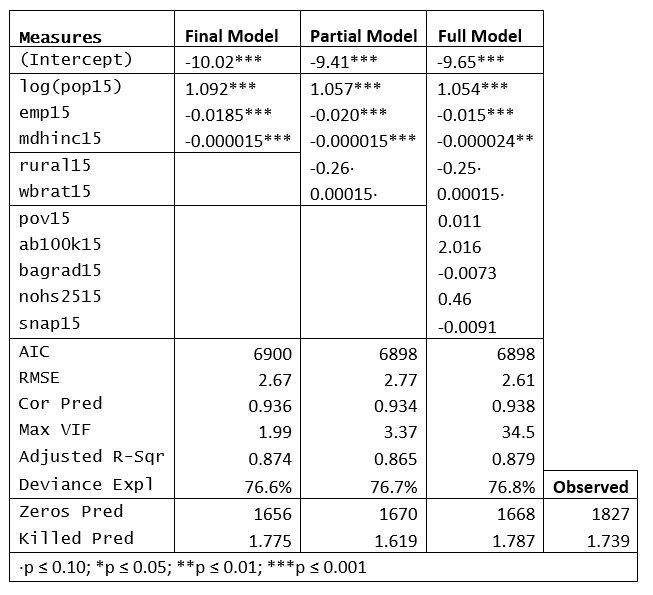
\includegraphics[width=1.0\textwidth]{images/table2.jpg}
\caption{Regression and diagnostic results from all three models.  "Zeros Pred" are the number of counties where no person is predicted to be killed by police, calculated not at exact zero, but any value less than 0.5.  "Killed Pred" is the mean number of predicted people killed by police in each county.}
\end{table}

The final regression model indicates a strong relationship between the dependent variable, the count of people killed by police in each county, and the three predictor variables, population of the county, employment rates in that county, and county median income.  The coefficients indicate both strength and direction of the relationship, and can be used to create a prediction equation. \\ 

Killed by Police = -10.01 + 1.092 * log(Population) - 0.0185 * Employment Rate - 0.000015 * Median Income\\

The coefficients imply that the higher a county's population, the higher the risk of being killed by police; the higher the employment rate in the county, the lower the risk of being killed by police; and the higher the county median income, the lower the risk of being killed by police.  The coefficients are interpreted as the change in the log-count killed by police for each unit change of the independent variables, presuming the other variables remain the same.  For practical purposes, this implies that taking the exponent of the predictor coefficient allows one to interpret the coefficients like a normal linear regression.  For example, as employment in a county rises by exp(0.0185), or 1.02\% it predicts a decrease of one count of police killing in that county.

The variance inflation factor did not indicate multicollinearity between these variables (max VIF=1.99). \cite{kaminski05,nix17} According to output from the R regression analysis, this three-variable model explains 76.6\% of the variance of the dependent variable, and the predicted vs observed killings by police have a correlation of 0.936.  The mean predicted killings are 1.78 per county, while the observed killings were 1.74.  This model predicts that 1,656 counties will have approximately zero killings (less than 0.5, not exactly zero), while the actual number of counties with no killings was 1,827. \cite{beaujean16}

Figures 3 shows two graphs supporting the conclusion that the final model is an acceptable fit.  The left plot of predicted versus observed killings by police per county, with the red regression line of just these two variables, shows the strong relationship between these two variables.  The rootogram on the right shows that few bins of predicted outcomes of the final model are significantly different from the observed values.  A rootogram is interpreted by the {\em hanging} bars--bars hanging above the zero-line are over-fit, while bars hanging below the line are under-fit. \cite{rootogram}  The closeness of the bars to the zero-line indicate a relatively good fit.

\begin{figure}
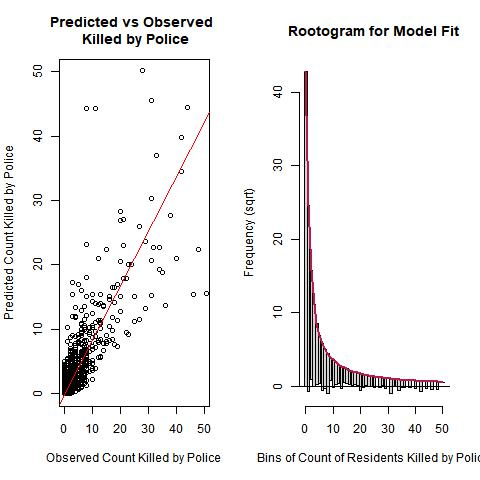
\includegraphics[width=1.0\textwidth]{images/figure3.jpg}
\caption{Left: Scatter plot of predicted versus observed counts of residents killed by police per county. Right: Rootogram--fit of the final regression model: negative binomial with three independent variables (log of population, employment and median income).  The red line can be interpreted as the observed values.  Bars that are hanging below the zero-line are under-fit for that bin, and those above the line are over-fit for that bin.}
\end{figure}

In addition to goodness of fit, regression also requires that residuals meet basic assumptions.  Figure 4 shows several standard diagnostic plots indicating that these assumptions seem to be met.  The residuals versus fitted values plot is interpreted as being problematic if a pattern emerges from the residuals, either above or below the zero-line.  In this case, no pattern is apparent--the residuals seem equally and randomly scattered above and below the line.  Similarly, the plot of residuals versus index shows a similar result, indicating the regression residuals assumption is met.  Finally, the bottom two plots, more residuals plots, show the same.  For example, the Normal Q-Q Plot would indicate a problem if a significant number of dots were straying from the main central line--in this case they are almost all on the line. \cite{hocking}

\begin{figure}
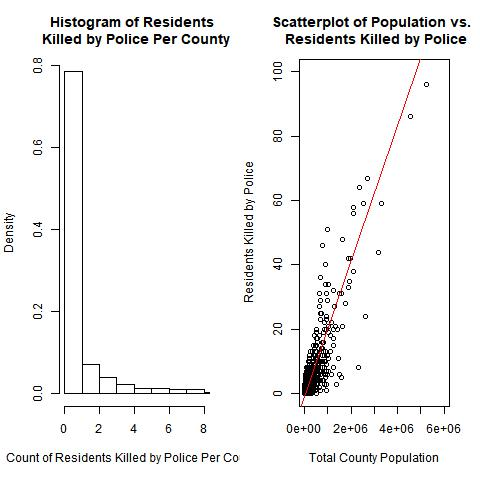
\includegraphics[width=1.0\textwidth]{images/figure4.jpg}
\caption{Regression diagnostics plots for the final model with three independent variables: population (log), employment and median income. Top: Residuals versus fitted and residuals versus index.  Bottom: Quantile residuals and QQ Plot of residuals. }
\end{figure}


\section{Conclusion}
The United States has an inordinate number of killings by law enforcement compared to other high-income countries.  People of color face the brunt of this violence as a share of the population.  Several theories have been proposed to explain these problems, such as minority threat, community inequality, police training, and citizen non-compliance.  One of the difficulties researching police violence is the lack of reliable data available to the public.  Until recently, the primary source for data was the FBI's Uniform Crime Report, which is widely known to be severely flawed.  Efforts by journalists and community activists have created several resources that are available to the public, and can be used for research on these types of killings.

Demographic, economic, political, and organizational variables can be analyzed with regression methods to model the types of social factors that are related to state violence.  A number of researchers have consistently found certain factors, like poverty, race and population density, to be related to levels of police violence.  Because counts are not normally distributed variables, negative binomial approaches have frequently been used for this type of data, and have produced consistent results.  Since the data that is available has been coded to many factors, including the specific location of the killing, mapping these deaths are possible.  This project used regression in R to model the relationship of several variables to killings by police, and mapping in QGIS to show county-level rates of violence in the United States, finding that the strongest, yet simplest model predicting police killings are the population size, employment rates, and median income.  This study did not look at any variables that could be considered individual, organizational, or situational, three theories commonly used to explain police violence.  However, the fact that two economic variables were significant predictors of deaths at the hands of law enforcement, would seem to contribute to the ecological approach, specifically, community economic structural factors.

\bibliographystyle{ACM-Reference-Format}
\bibliography{report} 

\end{document}
